\section{CUARTO TEMA}

De acuerdo con la ASCE 7-16 y la norma E.031 cuando se realice un análisis tiempo historia para diseñar edificaciones que incorporen algún sistema de control pasivo se debe usar un mínimo de siete registros sísmico, los cuales deben estar escalados correctamente. Dado que el objetivo de la presente tesis no es realizar un diseño detallado sino más bien conocer la eficiencia de cada sistema de control pasivo en la reducción de la respuesta sísmica, se usaron solo tres registros.

	\subsection{Registros Sísmicos Ajustados}
	
A continuación se presentan los registros sísmicos usados en la presente tesis.
			
	\begin{figure}[h!]
	\centering
	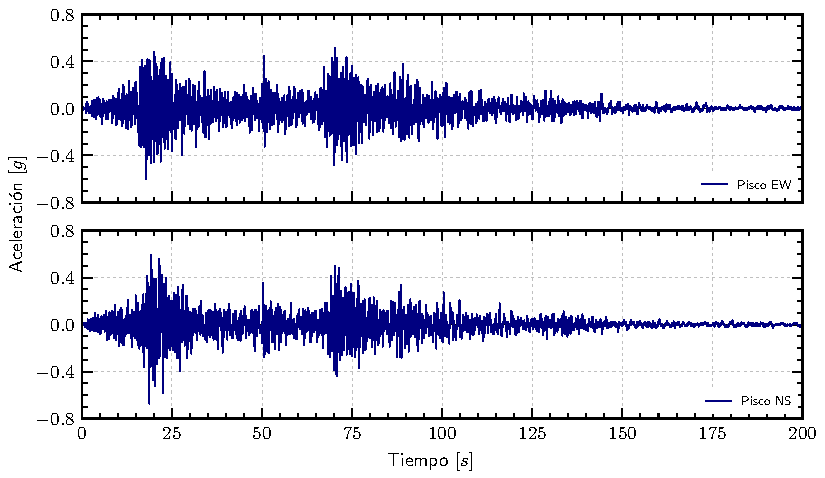
\includegraphics[scale=1]{E_IMAGENES/1_Capitulo2/Cap2_PiscoSc.pdf}
	\vspace{-8 mm}
	\caption[Acelerogramas espectrocompatibles - Pisco 2007]{\centering\footnotesize Acelerogramas espectrocompatibles - Pisco 2007.}
	\label{Cap2_Figura15}
	\end{figure}	
			
